%\documentclass[trans,handout]{beamer}
\documentclass[trans]{beamer}
\usetheme{eit}

%\usepackage{pgfpages}
%\pgfpagesuselayout{4 on 1}[a4paper,landscape,border shrink=5mm]
%\pgfpagesuselayout{2 on 1}[a4paper,border shrink=5mm]

\usepackage[utf8]{inputenc}
\usepackage{graphicx}
\usepackage{textpos}
\usepackage{textcomp}
\usepackage{floatrow}
\usepackage{multicol}
\usepackage{hyperref}
\hypersetup{
  colorlinks=true,
  linkcolor=black,
  urlcolor=blue
}
\graphicspath{{figures/}}

\title{
  
\includegraphics[height=.2\textheight]{../abstract/biopython.jpg}\\[1em]
  Biopython Project Update 2016}
\subtitle{}
\author[Christian Brueffer]{
  \textbf{Christian Brueffer}*, Tiago Ant\~{a}o, Peter Cock, Eric Talevich,\\
  Michiel de Hoon, Wibowo Arindrarto, Leighton Pritchard,\\
  Anuj Sharma, Eric Rasche, Aaron Rosenfeld, Connor T.\\
  Skennerton, Marco Galardini, Markus Piotrowski,\\
  and the Biopython Contributors}
\institute[Translational Oncogenomics Unit, Department of Clinical Sciences, Lund University]{* Twitter \& GitHub: @cbrueffer\\Translational Oncogenomics Unit\\Department of Clinical Sciences \\
  Lund University\\
  Sweden\\[1em]
  Bioinformatics Open Source Conference 2016, Orlando, USA \\[1em]
  %
\includegraphics[height=.2\textheight]{../abstract/biopython.jpg}
}
\date{July 9th, 2016}


\setcounter{tocdepth}{2}
\setbeamertemplate{caption}{\insertcaption}


% ToC at the beginning of every section
%\AtBeginSection[]
%{
 % \begin{frame} % with <beamer> => doesn't appear in handout mode
  %  \frametitle{Outline} %% Put the title you want, or none!
  %  \tableofcontents[currentsection,currentsection]
 % \end{frame}
%}

\begin{document}

%%%%%%%%%%%%%%%%%%%%%%%%%%%%%%%%%%%%%%%%%%%%%%%%%%%%%%%%%%%%%%%%%%%%%%%%%%%%%%%%
\begin{frame}
	\titlepage
\end{frame}
\setbeamertemplate{footline}[body]

\begin{frame}
    \frametitle{Outline}
    \tableofcontents
\end{frame}

%%%%%%%%%%%%%%%%%%%%%%%%%%%%%%%%%%%%%%%%%%%%%%%%%%%%%%%%%%%%%%%%%%%%%%%%%%%%%%%%

\section{The Biopython Project}
\frame
{
  \frametitle{What is Biopython?}

  \begin{itemize}
  \item Collection of modules for biological computation in Python
  \begin{itemize}
  \item Sequence handling and motifs, parsers, database queries, protein structures, phylogenetics, tool wrappers and lots more
  \end{itemize}
  \item Started in 1999, first release in 2000
  \item Open source and freely available (Biopython license)
  \end{itemize}

  \begin{center}
  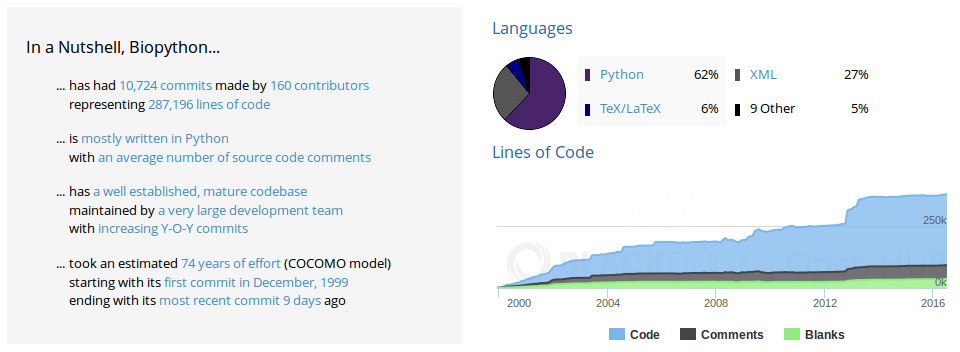
\includegraphics[width=1\textwidth]{openhub-bp-nutshell.png}
  \end{center}
  \small{Source: \url{https://www.openhub.net/p/biopython}}
}
\frame
{
  \frametitle{Stats for the previous 12 months}

  \begin{center}
  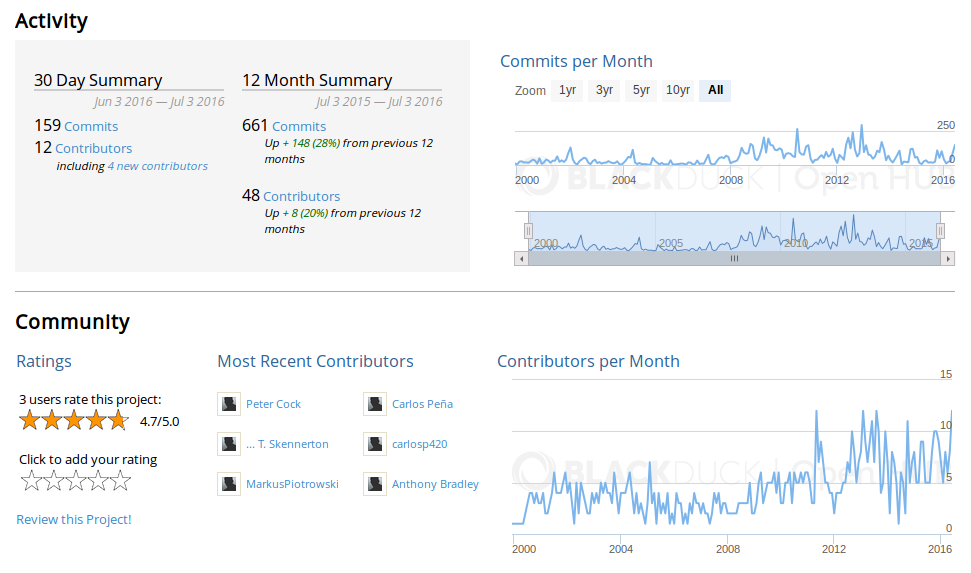
\includegraphics[width=1.0\textwidth]{openhub-bp-activity-community.png}
  \end{center}
  \small{Source: \url{https://www.openhub.net/p/biopython}}
}
\frame
{
  \frametitle{Lots of new contributors!}
  
  \scriptsize{
  \begin{multicols}{3}
  \begin{itemize}
  % 1.66
  \item Alan Medlar
  \item Anthony Mathelier
  \item Antony Lee
  \item Anuj Sharma
  \item Ben Fulton
  \item Bertrand Néron
  \item Connor T. Skennerton
  \item David Arenillas
  \item David Nicholson
  \item Emmanuel Noutahi
  \item Eric Rasche
  \item Fabio Madeira
  \item Franco Caramia
  \item Gert Hulselmans
  \item Gleb Kuznetsov
  \item John Bradley
  \item Kian Ho
  \item Kozo Nishida
  \item Kuan-Yi Li
  \item Sunhwan Jo
  \item Tarcisio Fedrizzi

  %1.67
  \item Aaron Rosenfeld
  \item Anders Pitman
  \item Barbara Mühlemann
  \item Ben Woodcroft
  \item Brian Osborne
  \item Chaitanya Gupta
  \item Chris Warth
  \item Christiam Camacho
  \item David Koppstein
  \item Jacek Śmietański
  \item João D Ferreira
  \item Joe Cora
  \item Marco Galardini
  \item Matt Ruffalo
  \item Matteo Sticco
  \item Nader Morshed
  \item Owen Solberg
  \item Steve Bond
  \item Terry Jones

  % after
  \item Anthony Bradley
  \item Uwe Schmitt
  \end{itemize}
  \end{multicols}
  }
}

%%%%%%%%%%%%%%%%%%%%%%%%%%%%%%%%%%%%%%%%%%%%%%%%%%%%%%%%%%%%%%%%%%%%%%%%%%%%%%%%

\section{New Releases and Beyond}
\subsection*{Release 1.66}
\frame
{
  \center{\LARGE Biopython 1.66 (released 2015-10-21)}
}

\frame
{
  \frametitle{Extended KEGG Plotting}
  
  \begin{itemize}
  \item Bio.KEGG and Bio.Graphics support transparency (Leighton Pritchard)
  \item \url{http://nbviewer.jupyter.org/github/widdowquinn/notebooks/blob/master/Biopython_KGML_intro.ipynb}
  \end{itemize}
  
  \begin{center}
  \includegraphics[width=1\textwidth]{kegg-ko0100.pdf}
  \end{center}
}

\frame
{
  \frametitle{Bio.SeqIO}
  
  \begin{itemize}
  \item Bio.SeqIO: Sequence input/output as SeqRecord objects  
  \item Extended ``abi'' Bio.SeqIO parser (Eric Rasche)
  \begin{itemize}
  \item appliedbiosystems ABIF format
  \item Now decodes almost all documented fields used by ABIF instruments
  \end{itemize}
  \end{itemize}
}

\frame
{
  \frametitle{Bio.PDB}
  
  \begin{itemize}
  \item Bio.PDB: Classes that deal with macromolecular crystal structures  
  \item New QCPSuperimposer module (Anuj Sharma)
  \begin{itemize}
  \item Additional option for superimposing structures
  \item Uses Quaternion Characteristic Polynomial algorithm
  \end{itemize}
  \end{itemize}
}

\frame
{
  \frametitle{Bio.Entrez}
  
  \begin{itemize}
  \item Bio.Entrez: Provides code to access NCBI over the WWW
  \item Better support for querying NCBI (Aaron Rosenfeld)
  \begin{itemize}
  \item Implement the NCBI Entrez Citation Matching function
  \item Support for NCBI XML files with XSD schemas
  \end{itemize}
  \end{itemize}  
}

\frame
{
  \frametitle{Miscellaneous}

  \begin{itemize}
  \item Python 2.6 support deprecated!
  \item Miscellaneous bug fixes
  \item Test suite enhancements
  \item Better PEP8 coding style adherence
  \end{itemize}
}

\frame
{
  \frametitle{Biopython 1.66 Contributors}

  \scriptsize{
  \begin{multicols}{2}
  \begin{itemize}
  \item Alan Medlar (*)
  \item Anthony Mathelier (*)
  \item Antony Lee (*)
  \item Anuj Sharma (*)
  \item Ben Fulton (*)
  \item Bertrand Néron (*)
  \item Brandon Invergo
  \item Carlos Pena
  \item Christian Brueffer
  \item Connor T. Skennerton (*)
  \item David Arenillas (*)
  \item David Nicholson (*)
  \item Emmanuel Noutahi (*)
  \item Eric Rasche (*)
  \item Fabio Madeira (*)
  \item Franco Caramia (*)
  \item Gert Hulselmans (*)
  \item Gleb Kuznetsov (*)
  \item João Rodrigues
  \item John Bradley (*)
  \item Kai Blin
  \item Kian Ho (*)
  \item Kozo Nishida (*)
  \item Kuan-Yi Li (*)
  \item Leighton Pritchard
  \item Lucas Sinclair
  \item Michiel de Hoon
  \item Peter Cock
  \item Saket Choudhary
  \item Sunhwan Jo (*)
  \item Tarcisio Fedrizzi (*)
  \item Tiago Antao
  \item Vincent Davis
  \end{itemize}
  \end{multicols}
  }
}

\subsection*{Release 1.67}
\frame
{
  \center{\LARGE Biopython 1.67 (released 2016-06-08)}
}

\frame
{
  \frametitle{Bio.SeqRecord module}
  
  \begin{itemize}
  \item Bio.SeqRecord: Represent a sequence with annotation
  \item Deprecation of ``=='' SeqRecord comparison (David Koppstein)
  \begin{itemize}
  \item Would return False even when SeqRecords had the same attributes
  \item Surprising for many users
  \end{itemize}
  \end{itemize}
}

\frame
{
  \frametitle{Bio.phenotype}
  
  \begin{itemize}
  \item Bio.phenotype: New module! (Marco Galardini)
  \item Support for working with Phenotype microarray data
  \item Parsing and analysis of cell culture growth measurements
  \begin{itemize}
  \item Data access (raw and interpolated)
  \item Curve fitting
  \item Parameter extraction
  \end{itemize}
  \item Writing PlateRecord objects as JSON (compatible with opm and DuctApe)
  \end{itemize}
}

\frame
{
  \frametitle{Bio.Restriction}
  
  \begin{itemize}
  \item Bio.Restriction: 
  \item REBASE May 2016 restriction enzyme list (Markus Piotrowski)
  \end{itemize}
}

\frame
{
  \frametitle{Bio.Data}
  
  \begin{itemize}
  \item Bio.Data: Collections of useful biological data (codon tables, alphabets, etc)
  \item Inclusion of NCBI genetic code table 25
  \begin{itemize}
  \item Candidate Division SR1
  \item Gracilibacteria
  \end{itemize}
  \end{itemize}
}

\frame
{
  \frametitle{BioSQL}
  
  \begin{itemize}
  \item BioSQL: SQL schema for biological sequence databases
  \item \url{http://biosql.org/}
  \item Updates to use foreign keys with SQLite3 databases (Connor T. Skennerton)
  \end{itemize}
}

\frame
{
  \frametitle{Miscellaneous}

  \begin{itemize}
  \item Python 3.3 support deprecated!
  \item Corrections to the Bio.Entrez module (Aaron Rosenfeld)
  \item Corrections to the MMCIF structure parser (João Rodrigues)
  \item Miscellaneous bug fixes
  \item Test suite enhancements
  \item Better PEP8 coding style adherence
  \end{itemize}
}

\frame
{
  \frametitle{Biopython 1.67 Contributors}

  \scriptsize{
  \begin{multicols}{2}
  \begin{itemize}
  \item Aaron Rosenfeld (*)
  \item Anders Pitman (*)
  \item Barbara Mühlemann (*)
  \item Ben Fulton
  \item Ben Woodcroft (*)
  \item Brandon Invergo
  \item Brian Osborne (*)
  \item Carlos Pena
  \item Chaitanya Gupta (*)
  \item Chris Warth (*)
  \item Christiam Camacho (*)
  \item Connor T. Skennerton
  \item David Koppstein (*)
  \item Eric Talevich
  \item Jacek Śmietański (*)
  \item João D Ferreira (*)
  \item João Rodrigues
  \item Joe Cora (*)
  \item Kai Blin
  \item Leighton Pritchard
  \item Lenna Peterson
  \item Marco Galardini (*)
  \item Markus Piotrowski
  \item Matt Ruffalo (*)
  \item Matteo Sticco (*)
  \item Nader Morshed (*)
  \item Owen Solberg (*)
  \item Peter Cock
  \item Steve Bond (*)
  \item Terry Jones (*)
  \item Vincent Davis
  \item Zheng Ruan
  \end{itemize}
  \end{multicols}
  }
}

\subsection*{Current Developments}
\frame
{
  \frametitle{1.68-dev}

  \begin{itemize}
  \item Module Bio.pairwise2 (pairwise sequence alignment) re-written (faster, addresses some problems with local alignments, and also now allows gap insertions after deletions, and vice versa) (Markus Piotrowski)

  \item The sample graphical tool SeqGui (Sequence Graphical User Interface) was
rewritten using the tkinter library (contributed by Markus Piotrowski). This
allows simple nucleotide transcription, back-transcription and translation
into amino acids using Bio.Seq internally, offering of the NCBI genetic codes
supported in Biopython. -> Markus Piotrowski

  \item NCBI Entrez and QBLAST API access through HTTPS rather than HTTP (Peter Cock)

  \item Bug fixes, further additions to the test suite, more Python PEP8 style adherence

  \end{itemize}
}


\frame
{
  \frametitle{Bio.PDB}
  
  \begin{itemize}
  \item Addition of RSSB's new Macromolecular Transmission Format (MMTF) (Anthony Bradley)
  \begin{itemize}
  \item Compressed binary format
  \item Better I/O attributes than PDB format
  \item $\Rightarrow$ Posters 21/22
  \end{itemize}
  \end{itemize}
}

\frame
{
  \frametitle{Bio.Data}
  
  \begin{itemize}
  \item Bio.Data: Collections of useful biological data
  \item Inclusion of NCBI genetic code table 26
  \begin{itemize}
  \item Pachysolen tannophilus Nuclear Code
  \end{itemize}
  \end{itemize}
}

%%%%%%%%%%%%%%%%%%%%%%%%%%%%%%%%%%%%%%%%%%%%%%%%%%%%%%%%%%%%%%%%%%%%%%%%%%%%%%%%

\section{Docker Images}
\frame
{
  \frametitle{Docker Images}

  \begin{itemize}
  \item Previously existing containers:
    \begin{itemize}
    \item container with Python 2/3, Biopython and all dependencies
    \item BioSQL container
  \end{itemize}
  \item New: Jupyter notebook containers
    \begin{itemize}
      \item basic version
      \item version including Biopython tutorial as notebooks
    \end{itemize}
  \end{itemize}
}

%%%%%%%%%%%%%%%%%%%%%%%%%%%%%%%%%%%%%%%%%%%%%%%%%%%%%%%%%%%%%%%%%%%%%%%%%%%%%%%%

\frame
{
  \frametitle{PEP8 Style}
  
  \begin{itemize}
  \item Widely different coding style in different modules in the past
  \item Large cleanup effort since 2012
  \item Git pre-commit hook (\url{https://github.com/cbrueffer/pep8-git-hook})
  \item Automatic style checking through TravisCI in preparation
  \end{itemize}
}

\section{General Updates}
\frame
{
  \frametitle{Continuous Integration}

  \begin{itemize}
  \item TravisCI
  \item Experimentation of different services
  \begin{itemize}
  \item Codecov.io (test coverage)
  \item Quantified Code (metrics and automatic pull requests)
  \item Landscape.io (``health score'')
  \end{itemize}
  \item Currently enabled by default: CodeCov.io
  \end{itemize}

  \begin{columns}
  \column{0.4\textwidth}
  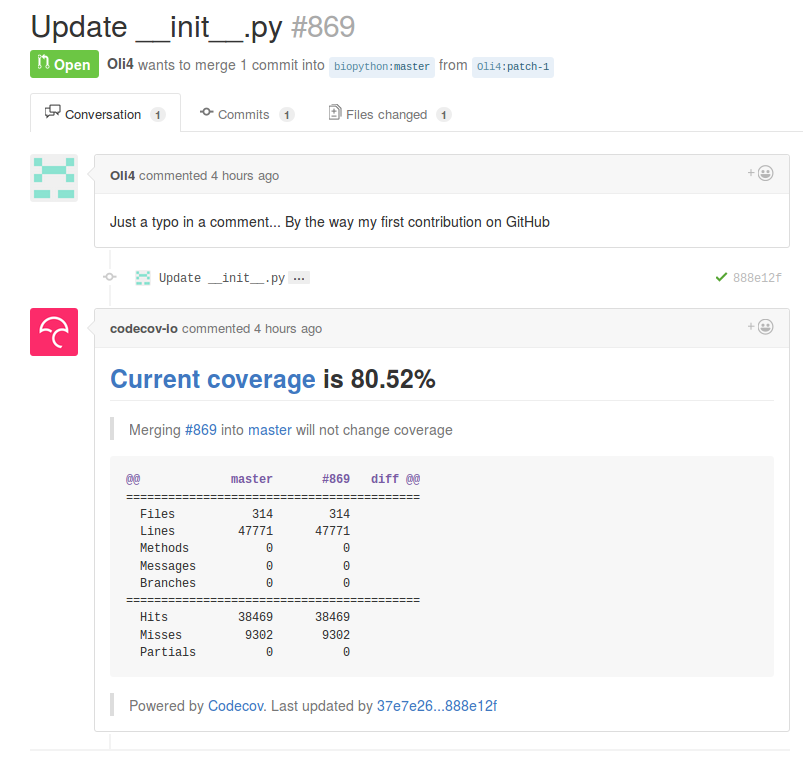
\includegraphics[width=1\textwidth]{bp-codecov.png}
  \column{0.6\textwidth}
  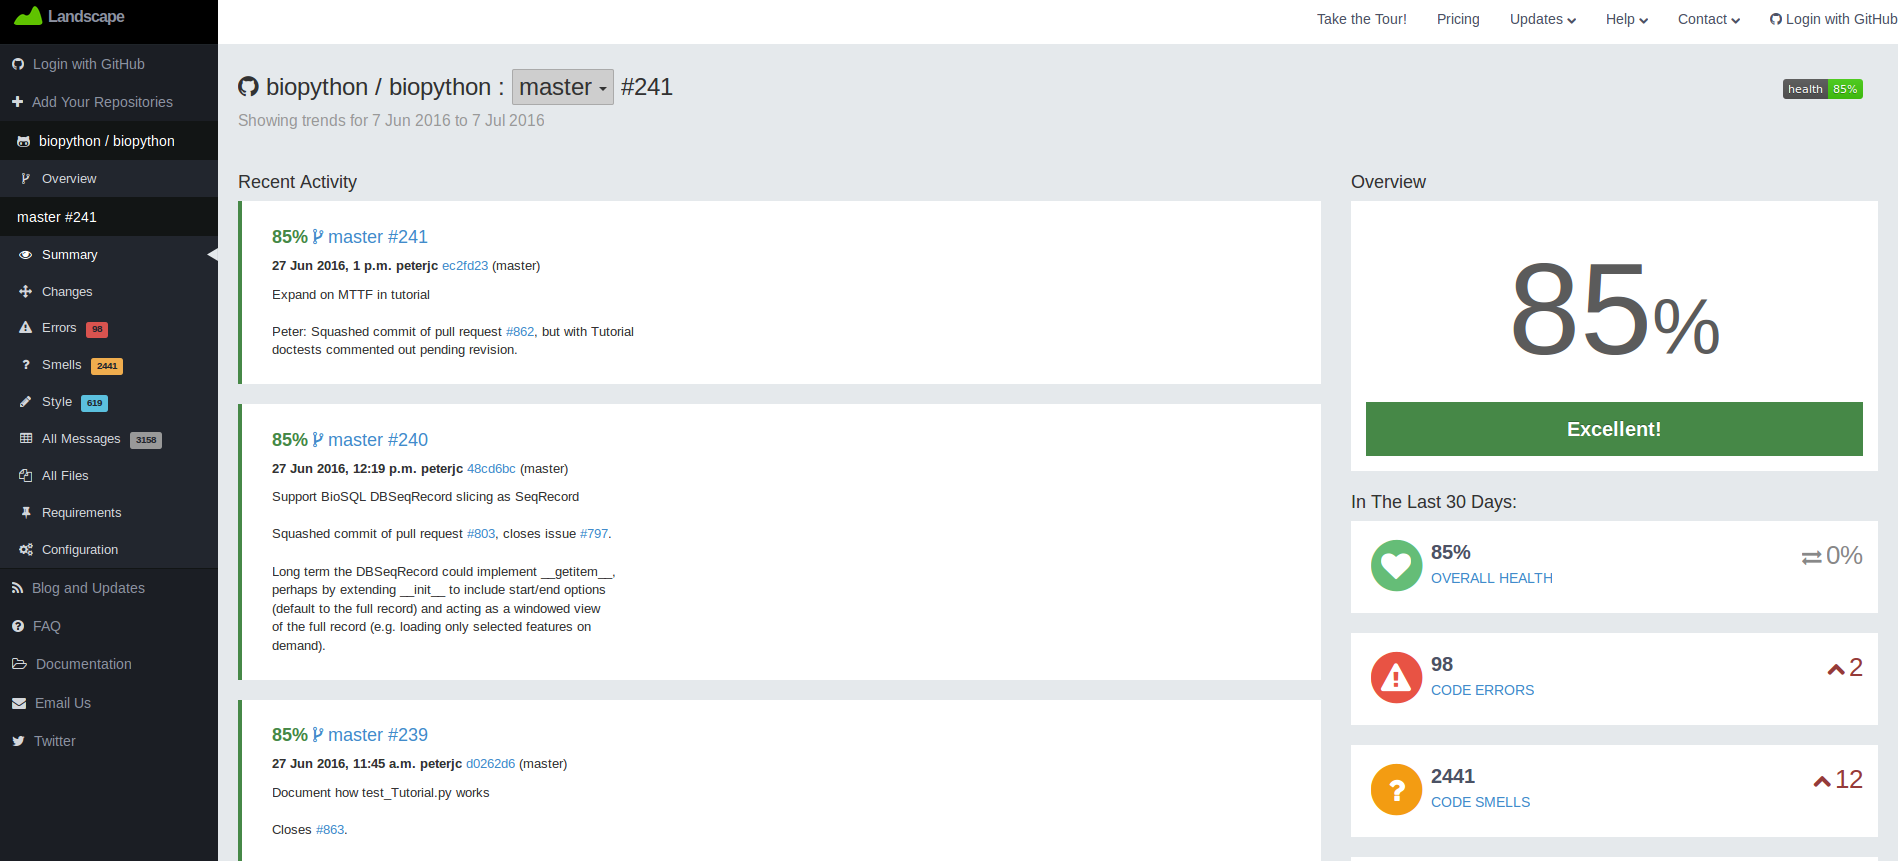
\includegraphics[width=1\textwidth]{bp-landscape.png}
  \end{columns}
}

\frame
{
  \frametitle{Website}

  \begin{itemize}
  \item Previously hosted by OBF until server problems
  \item Migrated from OBF MediaWiki to GitHub Pages
  \item Repository: \url{https://github.com/biopython/biopython.github.io}
  \end{itemize}

  \begin{center}
  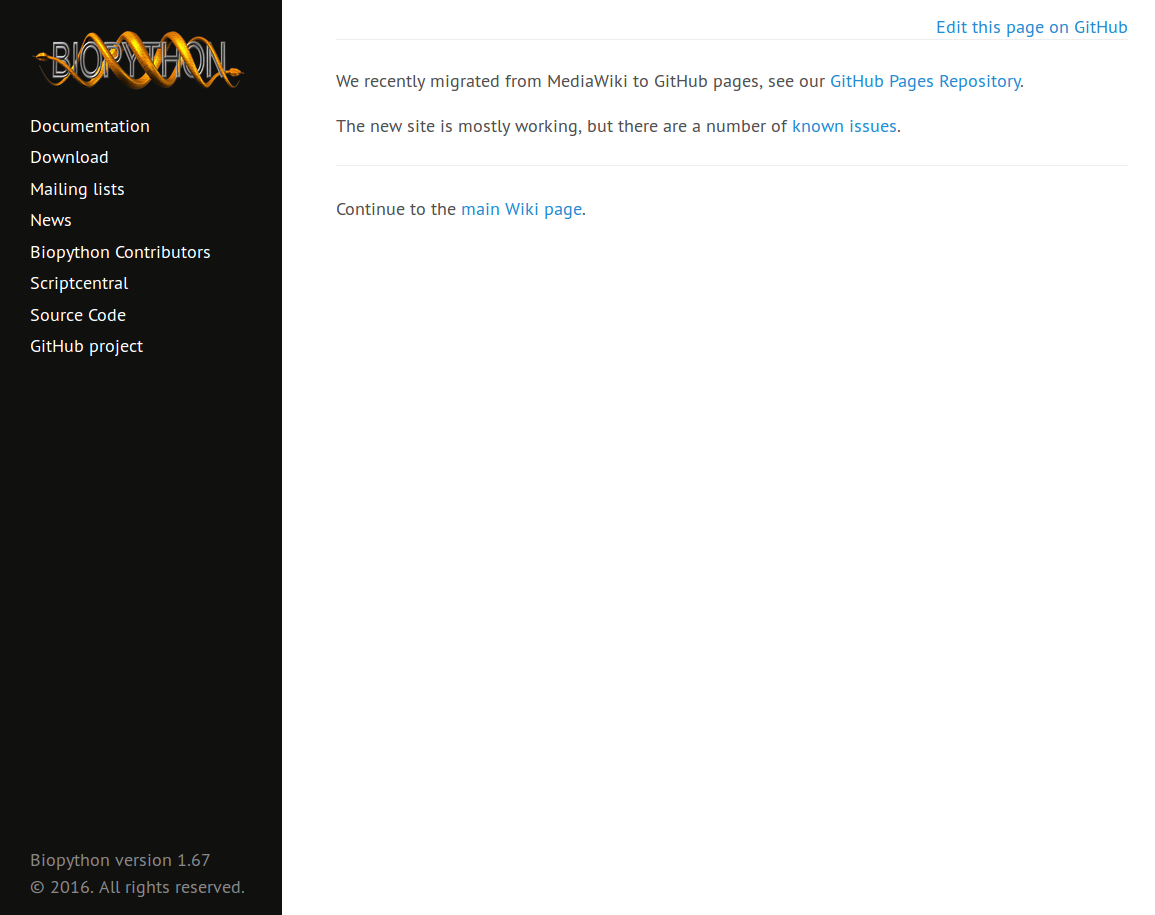
\includegraphics[width=0.9\textwidth]{bp-website.png}
  \end{center}
}

%%%%%%%%%%%%%%%%%%%%%%%%%%%%%%%%%%%%%%%%%%%%%%%%%%%%%%%%%%%%%%%%%%%%%%%%%%%%%%%%

\section{Conclusion}
\frame
{
  \frametitle{Conclusion}

  \begin{itemize}
  \item Lots of new stuff
  \item Lots of new contributors
  \end{itemize}
}

\section*{Acknowledgements}
\frame
{
  \frametitle{Resources!}

  %\begin{center}
  Website:\\
  \begin{itemize}
  \item \url{http://biopython.org}
  \end{itemize}

  Repositories:\\
  \begin{itemize}
  \item Main: \url{http://github.com/biopython/biopython}
  \item Docker: \url{http://github.com/biopython/biopython_docker}
  \item Website: \url{https://github.com/biopython/biopython.github.io}
  \end{itemize}

  Mailing lists:
  \begin{itemize}
  \item General list: \url{biopython@biopython.org}
  \item Developers list: \url{biopython-dev@biopython.org}
  \end{itemize}

  Biostars:
  \begin{itemize}
  \item \url{https://www.biostars.org/t/biopython/} (``biopython'' category)
  \end{itemize}
  %\end{center}
}

\frame
{
  \frametitle{Acknowledgements}

  \begin{minipage}{1\textwidth}
  \begin{columns}
  \column{0.5\textwidth}
  \begin{itemize}
  \item Peter Cock
  \item Biopython Community
  \end{itemize}
  \column{0.5\textwidth}
  
\includegraphics[width=0.8\textwidth]{../abstract/biopython.jpg}
  \end{columns}
  \end{minipage}

  \vspace{0.5cm}

  \begin{minipage}{1\textwidth}
  \begin{columns}
  \column{0.5\textwidth}
  \begin{itemize}
  \item Lao Saal (PhD supervisor)
  \item Faculty of Medicine
  \end{itemize}
  \column{0.5\textwidth}
  
\includegraphics[width=0.5\textwidth]{LundUniversity_C2line_PMS.eps}
  \end{columns}
  \end{minipage}
  
  \vspace{0.5cm}  
  
  \begin{minipage}{1\textwidth}
  \begin{columns}
  \column{0.2\textwidth}
  
\includegraphics[width=0.5\textwidth]{github-logo.jpg}
  \column{0.2\textwidth}
  
\includegraphics[width=0.5\textwidth]{travisci-logo.png}
  \column{0.2\textwidth}
  
\includegraphics[width=0.5\textwidth]{codecov-logo.png}
  \column{0.2\textwidth}
  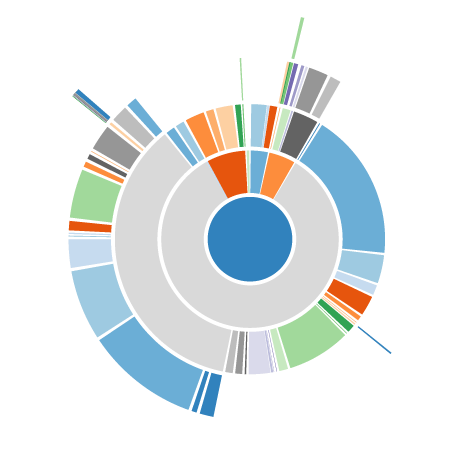
\includegraphics[width=0.5\textwidth]{quantifiedcode-logo.png}
  \column{0.2\textwidth}
  
\includegraphics[width=0.5\textwidth]{obf-logo.png}
  \end{columns}
  \end{minipage}
}

\end{document}